\documentclass[12pt]{article}

\usepackage{sbc-template}
\usepackage{graphicx,url}
\usepackage[utf8]{inputenc}
\usepackage[brazil]{babel}

\sloppy

\title{Análise Histórica do Sistema Operacional Linux:\\ do passatempo de um estudante à infraestrutura digital contemporânea}

\author{Lucas Henrique Lopes Costa\inst{1}, Pedro Gonçalves Costa Melo\inst{1},
  Thiago Lima\inst{1} \\
  André Mendonça\inst{1}, Tiago De Paula Martins\inst{1}, Gustavo de Jesus\inst{1} \\
  Luís Carlos Paiva\inst{1}, Samuel Moreira Abreu\inst{1} }

\address{Curso de Sistemas de Informação \\
  Universidade Federal de Lavras (UFLA) \\
  Lavras -- Minas Gerais -- Brasil
}

\begin{document}

\maketitle

\begin{abstract}
  This paper presents a historical and social analysis of the Linux operating
  system, from its emergence in 1991 as a personal project by the Finnish
  student Linus Torvalds to its consolidation as the foundation of contemporary
  digital infrastructure. Rather than merely describing technical features, it
  seeks to understand why such features came to be the way they are, recovering
  the motivations, conflicts and social decisions that shaped the project. It is
  argued that key technical choices, such as the monolithic kernel architecture
  and the adoption of the GNU GPL license, can only be explained in light of the
  collective and open development process that characterized Linux.
\end{abstract}

\begin{resumo}
  Este artigo realiza uma análise histórica e social do sistema operacional
  Linux, do seu surgimento em 1991, como projeto pessoal do estudante finlandês
  Linus Torvalds, até sua consolidação como base da infraestrutura digital
  contemporânea. Mais do que descrever características técnicas, busca-se
  compreender por que tais características vieram a existir do modo como existem,
  recuperando as motivações, os conflitos e as decisões sociais que moldaram o
  projeto. Argumenta-se que escolhas técnicas centrais, como a arquitetura
  monolítica do núcleo e a adoção da licença GNU GPL, só se explicam à luz do
  processo coletivo e aberto de desenvolvimento que caracterizou o Linux.
\end{resumo}

\section{Introdução}

Quando se propõe a análise histórica de uma tecnologia, o primeiro desafio é a
delimitação adequada do objeto. Categorias amplas, como ``tecnologia de
telecomunicação'' ou ``tecnologia de videogames'', não constituem, na verdade,
uma única tecnologia, mas conjuntos de inúmeras invenções com origens distintas.
O sistema operacional Linux, ao contrário, atende plenamente ao critério de uma
tecnologia bem delimitada: pode ser rastreado a um criador identificável, Linus
Benedict Torvalds, e a uma data inicial precisa, o ano de 1991. Há, portanto,
uma data de nascimento, uma ideia original e uma trajetória de desenvolvimento
passível de reconstrução \cite{moody2001}.

Este trabalho não se limita a descrever o que é ou como funciona o Linux. O
interesse central é o aspecto histórico e social: por que a ideia surgiu, quem a
teve, com que motivações, quais conflitos e parcerias marcaram seu
desenvolvimento e a que grupos sua difusão beneficiou ou prejudicou. Adota-se
aqui a premissa de que as características técnicas de qualquer artefato, embora à
primeira vista pareçam neutras, são sempre o resultado de um processo social.
Assim, ao longo do texto, as escolhas de engenharia do Linux serão
constantemente explicadas em função da história de sua criação, e nunca
isoladamente. O objetivo é mostrar, com um caso concreto, que a técnica nasce da
história, e que entender uma tecnologia exige entender as pessoas, os interesses
e os embates que a produziram.

\section{Contexto histórico: o início dos anos 1990 e o mundo Unix}

Para compreender o nascimento do Linux é preciso situar o momento histórico. No
início da década de 1990, os computadores pessoais tornavam-se cada vez mais
acessíveis, e os processadores de 32 bits, como o Intel 80386, traziam para a
mesa do usuário comum recursos antes restritos a máquinas de grande porte, tais
como a multitarefa real e a memória protegida. Ao mesmo tempo, o sistema
operacional Unix, criado nos laboratórios Bell na década de 1970, era a
referência técnica e conceitual dominante no meio acadêmico, porém estava
fragmentado em versões comerciais caras e de código fechado.

Existia, portanto, uma lacuna concreta: havia hardware poderoso e barato, havia
um modelo de sistema operacional admirado, o Unix, mas não havia um sistema
livre, completo e gratuito que aproveitasse esse hardware e pudesse ser estudado
e modificado livremente. É nessa lacuna, e não em um vazio, que o Linux aparece.
Ele surge primeiro como uma iniciativa pequena e pessoal, e não como um produto
pronto de mercado.

\section{A origem da ideia: Torvalds, o MINIX e o computador 386}

A ideia original do Linux não nasceu de um grande projeto institucional, mas da
frustração cotidiana de um estudante universitário. Em 1991, Linus Torvalds
tinha cerca de 21 anos e cursava Ciência da Computação na Universidade de
Helsinque, na Finlândia. Para estudar sistemas operacionais, utilizava o MINIX,
um sistema didático semelhante ao Unix desenvolvido pelo professor Andrew S.
Tanenbaum. O MINIX, porém, fora concebido como ferramenta de ensino: tinha
código de distribuição restrita, evoluía lentamente e não aproveitava plenamente
os recursos do hardware mais recente.

\begin{figure}[ht]
\centering
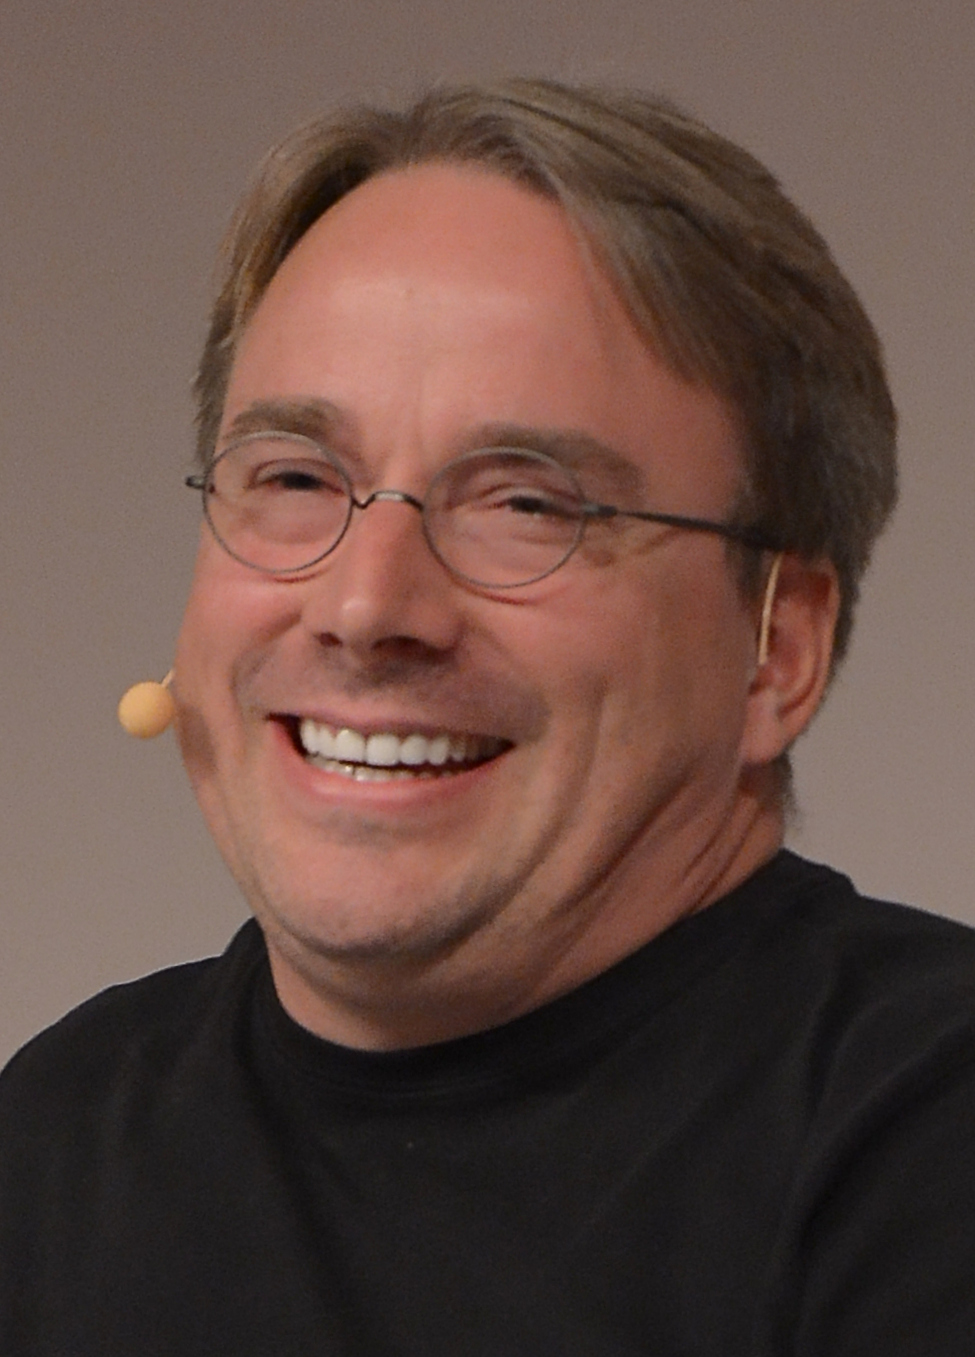
\includegraphics[width=.32\textwidth]{imgs/torvalds.jpg}
\caption{Linus Torvalds, criador do núcleo Linux, em conferência da Linux
  Foundation. Fonte: Wikimedia Commons (autor: Krd, licença CC BY-SA 4.0).}
\label{fig:torvalds}
\end{figure}

O estopim foi a compra de um computador pessoal com o então moderno processador
Intel 80386. Insatisfeito com as limitações do MINIX e desejando explorar a
fundo o seu novo equipamento, Torvalds começou a escrever, por conta própria,
pequenos programas para experimentar a troca de tarefas (multitarefa) do
processador. O que motivou a ideia, portanto, foi uma combinação de curiosidade
técnica, desejo de aprender fazendo e a recusa em aceitar as restrições do
software disponível. Não havia, no início, qualquer ambição comercial ou
consciência de que aquilo se tornaria relevante: tratava-se, em suas próprias
palavras, de um passatempo \cite{torvalds2001}.

\section{Objetivos iniciais e características desejadas}

Os objetivos iniciais do projeto eram modestos e pessoais. Torvalds queria um
sistema que rodasse bem em seu próprio hardware (a arquitetura 386), que fosse
semelhante ao Unix, cujo modelo conceitual ele admirava, e, sobretudo, que fosse
livre das amarras de licenciamento que o incomodavam no MINIX. As
características desejadas, nesse momento, derivavam diretamente dessas
motivações: um núcleo (kernel) eficiente, capaz de explorar a multitarefa do
386, e compatível com as ferramentas e a filosofia do mundo Unix.

É importante notar que a maior parte dessas características não foi planejada de
forma abstrata e antecipada, como ocorreria em um projeto de engenharia
tradicional. Elas emergiram de forma incremental, à medida que o autor resolvia
problemas concretos e adicionava funcionalidades conforme a necessidade, tais
como acessar o terminal, ler e gravar arquivos em disco e controlar processos.
Esse caráter pragmático e evolutivo é, ele próprio, uma característica social do
projeto, e não meramente técnica: explica por que o Linux cresceu por acréscimos
sucessivos em vez de seguir uma especificação rígida definida de antemão.

\section{O início do projeto e a sequência do desenvolvimento}

O projeto começou de modo quase acidental. Os primeiros programas de Torvalds
eram, na prática, um emulador de terminal para acessar os servidores Unix da
universidade. Aos poucos, ao acrescentar rotinas para ler e gravar arquivos em
disco e gerenciar o hardware, esse emulador foi se transformando em algo muito
maior: o embrião de um núcleo de sistema operacional.

Um marco simbólico da história ocorreu em 25 de agosto de 1991, quando Torvalds
publicou uma mensagem no grupo de discussão da Usenet \texttt{comp.os.minix}
anunciando que estava desenvolvendo um sistema operacional livre. Nas suas
palavras, era ``apenas um passatempo'' (\textit{just a hobby}), que não seria
``grande e profissional como o GNU'' \cite{torvalds1991}. A frase, hoje célebre
por sua modéstia diante do que viria a acontecer, convidava outros usuários a
opinarem sobre o que gostariam de ver no sistema. Em setembro de 1991, foi
disponibilizada a versão 0.01 em um servidor FTP.

Curiosamente, o próprio nome do sistema resultou de uma decisão alheia ao autor.
Torvalds pretendia chamá-lo de ``Freax'', combinação de \textit{free},
\textit{freak} e a letra ``x'' de Unix. Contudo, o administrador do servidor FTP
onde o código foi hospedado nomeou o diretório como ``linux'', e foi esse o nome
que se popularizou \cite{torvalds2001}. Trata-se de um exemplo claro de como
fatores contingentes e sociais, e não apenas a vontade do criador, moldam o
destino de uma tecnologia. Posteriormente, a comunidade adotaria como mascote o
pinguim Tux (Figura~\ref{fig:tux}), desenhado por Larry Ewing em 1996 com o
software livre GIMP, reforçando a identidade coletiva do projeto.

\begin{figure}[ht]
\centering

\includegraphics[width=.20\textwidth]{imgs/tux.png}
\caption{Tux, o pinguim que se tornou mascote oficial do Linux. Fonte: Wikimedia
  Commons (autor: Larry Ewing, lewing@isc.tamu.edu, e The GIMP).}
\label{fig:tux}
\end{figure}

Os passos seguintes para viabilizar o projeto foram dados não por Torvalds
isoladamente, mas por uma rede crescente de colaboradores espalhados pelo mundo,
que enviavam correções e melhorias pela internet. A sequência de versões avançou
rapidamente: a versão 1.0, considerada a primeira estável e completa, foi
lançada em março de 1994; a versão 2.0, de 1996, já trazia suporte a múltiplos
processadores \cite{moody2001}. O ritmo acelerado de evolução só foi possível
graças ao modelo de desenvolvimento aberto, descrito adiante.

\section{Aliados, financiamento e o Projeto GNU}

A pergunta sobre quem foram os aliados do projeto revela o aspecto mais decisivo
da história do Linux. O principal parceiro não foi uma pessoa ou empresa
específica, mas um modelo de colaboração: a comunidade global de desenvolvedores
voluntários que, conectada pela internet emergente, passou a contribuir com o
código. Esse arranjo permaneceu até hoje e é a razão de o Linux jamais ter
dependido de um único agente. Vale destacar a questão do financiamento, pois
nenhum projeto avança sem recursos. No caso do Linux, o ``capital'' inicial não
foi dinheiro, mas o tempo doado por milhares de programadores e a infraestrutura
gratuita de comunicação oferecida pela internet acadêmica. Só mais tarde viria o
financiamento corporativo direto.

\begin{figure}[ht]
\centering
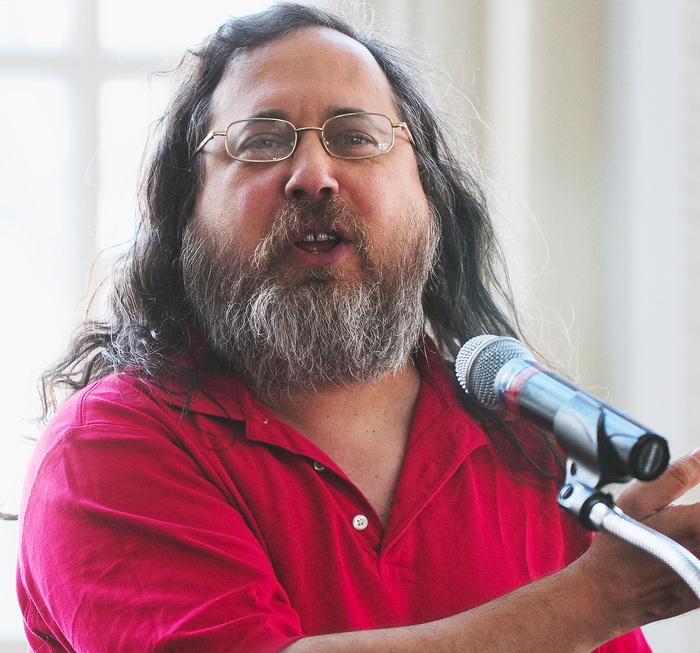
\includegraphics[width=.30\textwidth]{imgs/stallman.jpg}
\caption{Richard Stallman, fundador do Projeto GNU e da Free Software
  Foundation, cujas ferramentas e licença foram decisivas para o Linux. Fonte:
  Wikimedia Commons (licença Creative Commons).}
\label{fig:stallman}
\end{figure}

Houve, ainda, uma aliança histórica fundamental, ainda que indireta. Desde 1983,
o programador Richard Stallman (Figura~\ref{fig:stallman}) conduzia o Projeto
GNU, cujo objetivo era construir um sistema operacional completo e totalmente
livre, semelhante ao Unix \cite{stallman_gnu}. Por volta de 1991, o GNU já
possuía praticamente todas as ferramentas necessárias, tais como o compilador,
os interpretadores de comandos e os utilitários, mas lhe faltava justamente a
peça central: um núcleo funcional, pois o núcleo próprio do projeto, o GNU Hurd,
não avançava. O Linux surgiu exatamente para preencher essa lacuna. A união do
núcleo de Torvalds com as ferramentas do GNU resultou em um sistema operacional
completo e livre, o que originou inclusive a controvérsia sobre a denominação
``GNU/Linux'', defendida por Stallman e pela Free Software Foundation
\cite{stallman_linuxgnu}.

Nem todos os agentes permaneceram em harmonia. O próprio Tanenbaum, autor do
MINIX que inspirou o projeto, tornou-se um crítico contundente, como se verá.
Ainda assim, a base comunitária se manteve coesa e expandiu-se com a formação de
empresas e fundações dedicadas ao sistema. Esse processo de institucionalização
culminou, em 2007, na criação da Linux Foundation, resultado da fusão entre o
Open Source Development Labs e o Free Standards Group, que passou a coordenar e
financiar parte do desenvolvimento, mantendo inclusive o salário do próprio
Torvalds \cite{lf_about}.

\section{Conflitos, críticas e mudanças de rumo}

O desenvolvimento do Linux enfrentou problemas técnicos e, sobretudo, problemas
de natureza jurídica e organizacional. No campo técnico, destaca-se o famoso
debate ocorrido no início de 1992 entre Torvalds e Andrew Tanenbaum, na Usenet,
sob o título provocador ``LINUX is obsolete'' (``o Linux é obsoleto'')
\cite{tanenbaum1992}. Tanenbaum, representante da visão acadêmica dominante,
sustentava que o sistema adotava uma arquitetura ultrapassada, o núcleo
monolítico, em vez do então prestigiado modelo de micronúcleo, e criticava sua
forte vinculação ao processador 386.

\begin{figure}[ht]
\centering
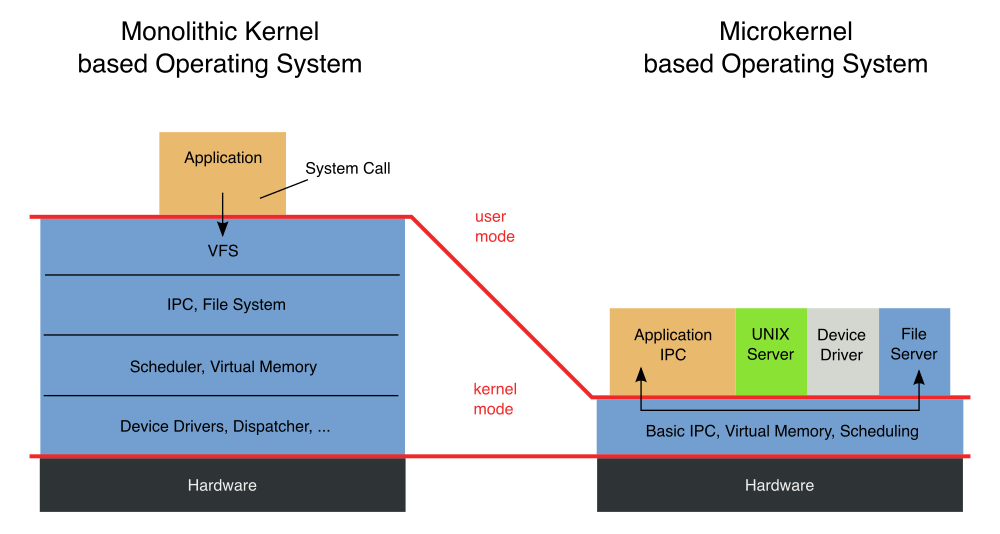
\includegraphics[width=.85\textwidth]{imgs/os-structure.png}
\caption{Diferença estrutural entre o núcleo monolítico, defendido por Torvalds,
  e o micronúcleo, defendido por Tanenbaum. No modelo monolítico, os serviços do
  sistema executam juntos no espaço do núcleo, o que favorece o desempenho.
  Fonte: Wikimedia Commons (arquivo OS-structure.svg).}
\label{fig:kernel}
\end{figure}

A Figura~\ref{fig:kernel} ilustra a diferença em disputa. No núcleo monolítico,
serviços como sistema de arquivos, gerência de memória e controladores de
dispositivo executam todos no mesmo espaço privilegiado, o que tende a ser mais
rápido; no micronúcleo, esses serviços são separados em módulos isolados, o que
favorece a portabilidade e a robustez, ao custo de desempenho. Torvalds defendeu
sua escolha com base no pragmatismo e na velocidade de desenvolvimento. Esse
episódio mostra com nitidez como uma característica técnica, a arquitetura do
núcleo, foi objeto de uma disputa social entre uma corrente acadêmico-purista e
uma corrente pragmática.

A mudança de rumo mais importante, contudo, foi de ordem legal. A primeira
licença do Linux, redigida pelo próprio Torvalds, proibia a cobrança por sua
distribuição. Essa restrição, paradoxalmente, limitava a adoção do sistema. Em
1992, Torvalds tomou a decisão que talvez tenha sido a mais relevante de toda a
sua trajetória: relicenciar o Linux sob a GNU General Public License (GPL), a
licença criada por Stallman \cite{gpl2}. A GPL garantia que o software
permanecesse livre, mas permitia seu uso comercial, desde que as modificações
também fossem compartilhadas. Essa alteração, uma decisão social e política, e
não técnica, destravou a colaboração massiva e o surgimento de um ecossistema
econômico em torno do sistema.

Cabe então responder se as características do produto final corresponderam ao que
se previa no início. A resposta é claramente negativa, e de forma positiva: o
Linux superou em muito qualquer expectativa de seu criador. O que nasceu como um
experimento pessoal para um único computador tornou-se um sistema portável,
executado em praticamente todas as arquiteturas de hardware existentes. Essa
portabilidade não estava no plano original, surgiu por demanda da comunidade. Do
mesmo modo, a rígida arquitetura monolítica foi flexibilizada com a introdução
dos módulos de núcleo carregáveis, em meados da década de 1990, conciliando
desempenho e modularidade. As mudanças, portanto, foram impulsionadas pelas
necessidades coletivas dos usuários e colaboradores.

\section{As características técnicas como produto de um processo social}

A trajetória do Linux ilustra de maneira exemplar a tese de que características
técnicas resultam de processos sociais. O modelo de desenvolvimento aberto foi
sintetizado pelo programador Eric S. Raymond, em 1997, no ensaio ``A Catedral e
o Bazar'' \cite{raymond2000}. Raymond contrapôs o modelo tradicional e fechado de
produção de software, a ``catedral'', construída por poucos especialistas em
segredo, ao modelo do Linux, o ``bazar'', caótico, público e colaborativo, em
que múltiplos olhos revisam o código continuamente. O lema de que ``com olhos
suficientes, todos os erros são superficiais'' explica, em termos sociais, por
que o Linux atingiu alta confiabilidade técnica.

Esse modelo deu origem, em 1998, ao próprio termo ``código aberto'' (\textit{open
source}), cunhado em parte como estratégia para tornar a filosofia do software
livre mais palatável ao mundo empresarial \cite{osi_history}. Assim, mesmo a
forma como o Linux é nomeado, licenciado e divulgado é fruto de escolhas sociais
deliberadas. A arquitetura monolítica, a licença GPL, a portabilidade e a
modularidade não são propriedades naturais do sistema: são respostas a
frustrações, debates, demandas e estratégias humanas concretas. Esse caráter
coletivo permanece visível nos números atuais do desenvolvimento, em que milhares
de programadores de mais de mil empresas diferentes contribuem a cada ano para o
núcleo \cite{kernel_about}.

\section{Beneficiados, prejudicados e disputas econômicas}

A difusão do Linux beneficiou amplos grupos. Desenvolvedores e estudantes
ganharam acesso gratuito ao código de um sistema operacional profissional,
transformando-o em poderosa ferramenta de aprendizado. Empresas e governos
passaram a dispor de uma alternativa robusta e de baixo custo, livre da
dependência de um único fornecedor, o chamado \textit{vendor lock-in}. Países em
desenvolvimento e instituições com poucos recursos puderam montar
infraestruturas tecnológicas sem o ônus de licenças caras.

Quanto aos grupos prejudicados, os mais evidentes são as empresas de software
proprietário, cujo modelo de negócio baseado na venda de licenças foi diretamente
desafiado. Não por acaso, no início dos anos 2000, executivos do setor chegaram a
classificar o modelo da GPL como uma ameaça ao seu negócio. Esse atrito revela um
deslocamento econômico importante: o software livre não significa ausência de
mercado, mas muda a forma como o valor e o lucro são gerados, deslocando-os da
venda da licença para serviços, suporte e infraestrutura.

Há ainda críticas internas. Parte da comunidade questiona se o trabalho
voluntário não seria, por vezes, apropriado gratuitamente por grandes
corporações que lucram com o esforço coletivo, o que abre um debate sobre
exploração e sustentabilidade do modelo. A fragmentação em inúmeras
distribuições e a histórica complexidade de uso para o público leigo também são
apontadas como pontos negativos, que limitaram a adoção do Linux nos
computadores pessoais domésticos.

\section{Impactos sociais e a infraestrutura digital contemporânea}

O balanço dos impactos é expressivo. No lado positivo, o Linux tornou-se a
espinha dorsal da computação moderna. Um dado sintetiza essa posição: desde
novembro de 2017, a totalidade dos 500 supercomputadores mais potentes do mundo
executa Linux, situação que se mantém ano após ano \cite{top500,lf_super}. No
mesmo sentido, a maior parte dos servidores que sustentam a web funciona sobre
Linux, que responde por mais de 60\% dos sítios cujo sistema operacional pode ser
identificado \cite{w3techs}.

O alcance é ainda maior quando se considera o usuário comum, muitas vezes sem que
ele perceba. O sistema Android, construído sobre o núcleo Linux, é a plataforma
móvel dominante no planeta, com cerca de 70\% do mercado mundial de smartphones
\cite{statcounter_mobile,android_kernel}. Ou seja, mesmo quem nunca instalou uma
distribuição Linux em um computador pessoal provavelmente utiliza o sistema
indiretamente todos os dias, ao usar o celular, acessar uma página na internet ou
um serviço em nuvem. O Linux, portanto, teve mais sucesso como infraestrutura
invisível do que como sistema popular de desktop.

No lado negativo, persistem a curva de aprendizado elevada para usuários comuns,
a fragmentação do ecossistema em muitas distribuições e as tensões sobre a
sustentabilidade do trabalho voluntário. Ainda assim, é difícil encontrar
tecnologia de software com alcance social comparável. Além do impacto direto, o
Linux consolidou a viabilidade econômica e cultural do software livre e
influenciou um método de produção colaborativa que extrapolou a informática,
inspirando iniciativas em áreas tão diversas quanto a ciência aberta e a cultura
livre.

\section{Considerações finais}

A história do Linux demonstra que uma das tecnologias mais influentes da era
digital nasceu de um gesto modesto: a insatisfação de um estudante com as
ferramentas de que dispunha. Sua trajetória, porém, só pode ser compreendida em
sua dimensão social. As decisões aparentemente técnicas, como a arquitetura do
núcleo, a licença adotada e a abertura do código, foram, na realidade, decisões
sociais e políticas que determinaram o sucesso do projeto.

Mais do que um sistema operacional, o Linux consolidou um método de produção
colaborativa do conhecimento. Analisar sua história é, em última instância,
perceber que a tecnologia nunca é apenas máquina ou código: ela é também
organização social, disputa econômica, decisão política e produção coletiva. O
Linux é, nesse sentido, o reflexo das pessoas, dos conflitos e das escolhas que o
produziram.

\bibliographystyle{sbc}
\bibliography{artigo-linux}

\end{document}
